\documentclass{beamer}

\usepackage[british]{babel}
\usepackage{graphicx,hyperref,ru,url}
\usepackage{amsmath}
\usepackage{qrcode}
\usepackage{hyperref}

% The title of the presentation:
%  - first a short version which is visible at the bottom of each slide;
%  - second the full title shown on the title slide;
\title[VII meeting - 2019]{Artificial Neural networks for the prediction of phage protein function }

% Optional: a subtitle to be dispalyed on the title slide
%\subtitle{Show where you're from}

% The author(s) of the presentation:
%  - again first a short version to be displayed at the bottom;
%  - next the full list of authors, which may include contact information;
\author[A. Cantu]{Adrian Cantu}

% The institute:
%  - to start the name of the university as displayed on the top of each slide
%    this can be adjusted such that you can also create a Dutch version
%  - next the institute information as displayed on the title slide
\institute[]{
  San Diego State University \\
  Computational Science Research Center}

% Add a date and possibly the name of the event to the slides
%  - again first a short version to be shown at the bottom of each slide
%  - second the full date and event name for the title slide
\date[03/23/2019]{
  March 23th 2019}

\begin{document}

\begin{frame}
  \titlepage
  \centering
\end{frame}


\begin{frame}{BacterioPhage}
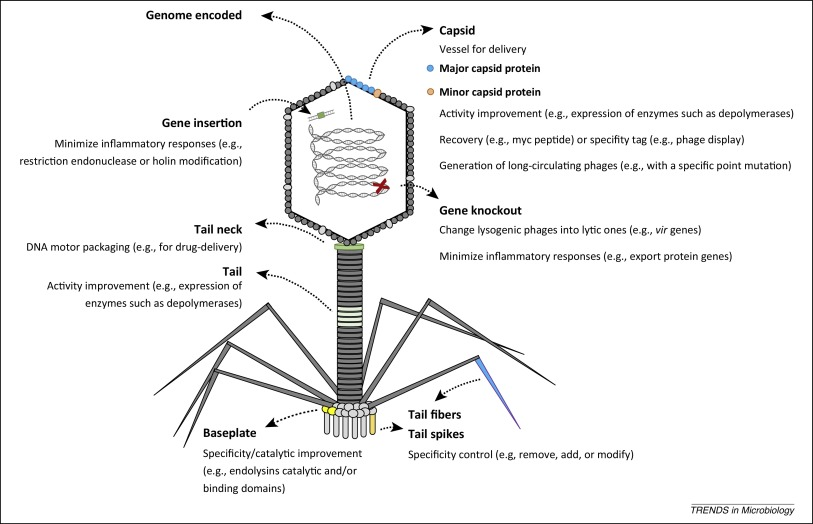
\includegraphics[width=0.90\textwidth]{img01}
\end{frame}

\begin{frame}{Databases}
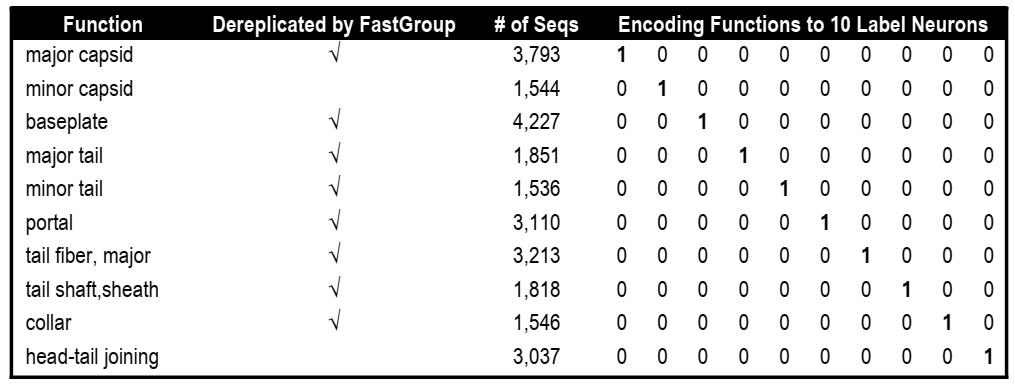
\includegraphics[width=0.90\textwidth]{img02_databases}
\end{frame}

\begin{frame}{Protein Sequences}
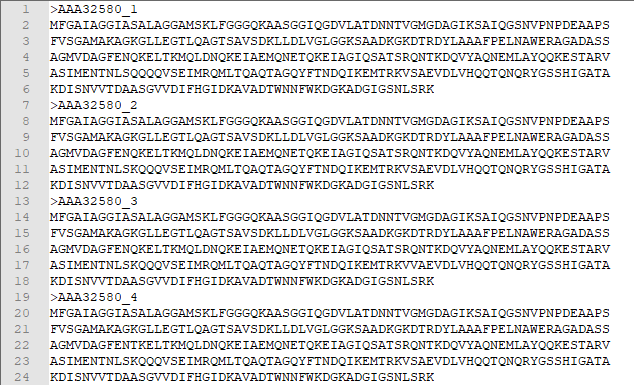
\includegraphics[width=0.90\textwidth]{fasta}
\end{frame}

\begin{frame}{F:Sequence --$>$ Function}
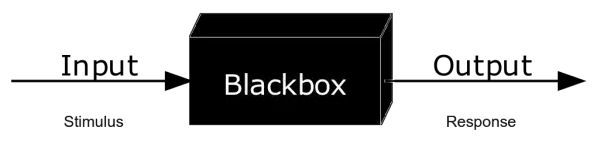
\includegraphics[width=0.90\textwidth]{blackbox}
\end{frame}

\begin{frame}{Artificial Neural Networks}
\begin{minipage}[t]{0.5\textwidth}
  \centering\raisebox{\dimexpr \baselineskip-\height}{%
  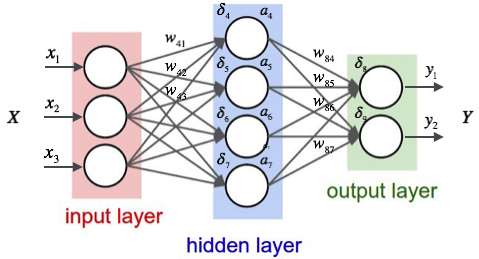
\includegraphics[width=0.90\textwidth]{img03_ANN}}
\end{minipage}\hfill
\begin{minipage}[t]{0.5\textwidth}
ANN have been shown to be universal approximators of \underline{continuous} functions in $\mathbb{R}^n$ \\
$$
d=\left(\int_0^{2\pi}|f_1(t)-f_2(t)|^p dt\right)^\frac{1}{p}
$$
where $1<p<\infty$
\end{minipage}
\end{frame}


\begin{frame}{Artificial Neural Networks}
\begin{minipage}[t]{0.5\textwidth}
$$
\begin{pmatrix}
Z_1\\ 
Z_2\\ 
\vdots \\ 
\vdots\\ 
\vdots\\ 
\vdots\\ 
\vdots\\ 
Z_{410}\\ 
\end{pmatrix}
\begin{matrix}
\\ 
\\ 
\\ 
\\ 
=X\\ 
\\ 
\\ 
\\ 
\\
\end{matrix}
$$
\end{minipage}\hfill
\begin{minipage}[t]{0.5\textwidth}
$$
\begin{pmatrix}
Y_1\\ 
Y_2\\ 
Y_3\\ 
Y_4\\ 
Y_5\\ 
Y_6\\ 
Y_7\\ 
Y_8\\ 
Y_{9}\\ 
Y_{10}
\end{pmatrix}
\begin{matrix}
\\ 
\\ 
\\ 
\\ 
\\ 
=Y\\ 
\\ 
\\ 
\\ 
\\ 
\\ 
\end{matrix}
$$
where $\sum_{n=1}^{10}Y_n=1$
\end{minipage}
\end{frame}

\begin{frame}{The 'black box' function}
\scalebox{0.7}{%
$F(X)=\underbrace{[10*200]}_{W_3}\left(\underbrace{[200*200]}_{W_2}\left(\underbrace{[200*407]}_{W_1}\underbrace{[407*1]}_X+\underbrace{[200*1]}_{\delta_1}\right)+\underbrace{[200*10]}_{\delta_2}\right)+\underbrace{[10*1]}_{\delta_1}
$} \\
\begin{center}
289,866 Trainable parameters
\end{center}
\end{frame}

\begin{frame}{Accuracy}
$$
\begin{matrix}
 & Precision & Recall & f1-score & Support\\ 
Major\ capsid & 0.91 & 0.79 & 0.85 & 95\\ 
Minor\ capsid & 0.78 & 0.93 & 0.85 & 45\\ 
Baseplate & 0.72 & 0.91 & 0.80 & 108\\ 
Major\ tail & 0.91 & 0.67 & 0.77 & 43\\ 
Minor\ Tail & 0.93 & 0.93 & 0.93 & 44\\ 
Portal & 0.92 & 0.81 & 0.86 & 80\\ 
Tail\ Fiber & 0.78 & 0.41 & 0.53 & 96\\  
Tail\ shaft & 0.70 & 0.72 & 0.71 & 39\\ 
Collar & 0.39 & 0.83 & 0.53 & 53\\ 
Head-Tail\ Joining & 0.98 & 0.98 & 0.98 & 90\\ 
 &  &  &  & \\ 
weighted\ avg & 0.82 & 0.79 & 0.79 & 675 
\end{matrix}
$$
\end{frame}



\begin{frame}{Results Confusion matrix}
\scalebox{0.95}{%
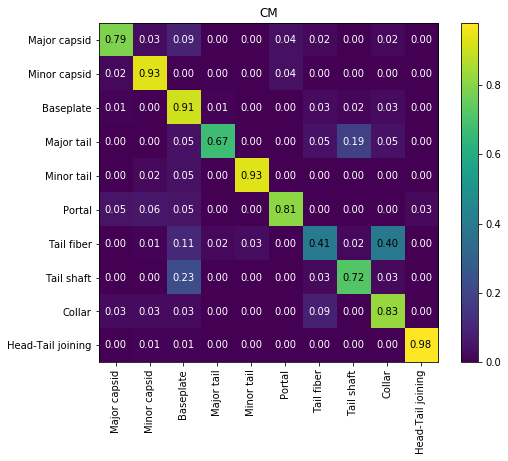
\includegraphics[width=0.90\textwidth]{confusion_mat}
}
\end{frame}

\begin{frame}{Weighted average}
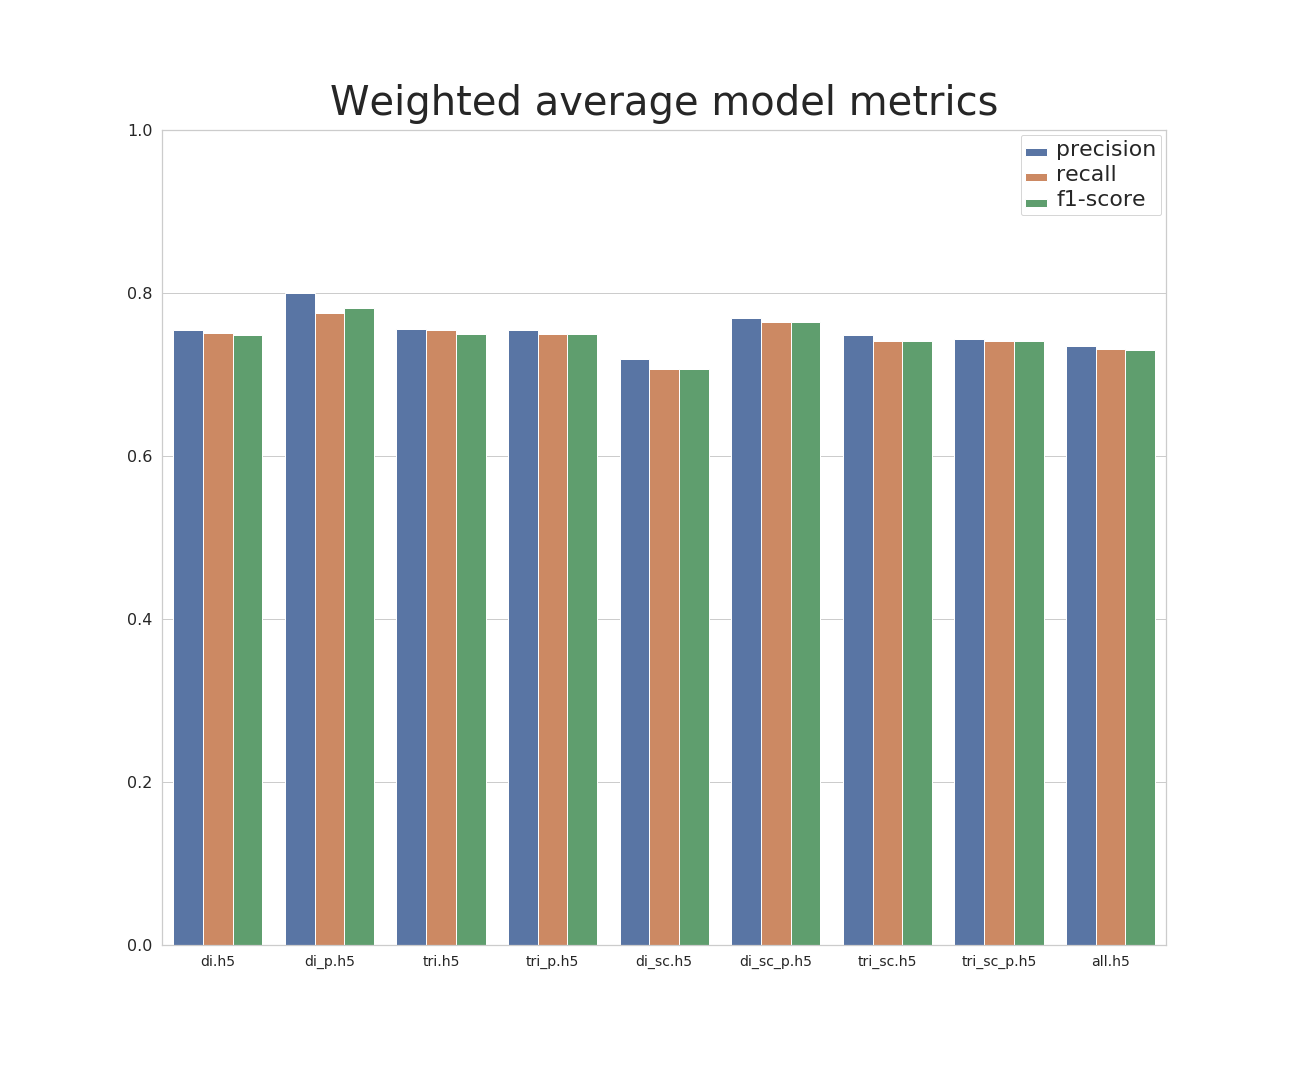
\includegraphics[width=0.90\textwidth]{avg_score}
\end{frame}

\begin{frame}{Per class f1-score}
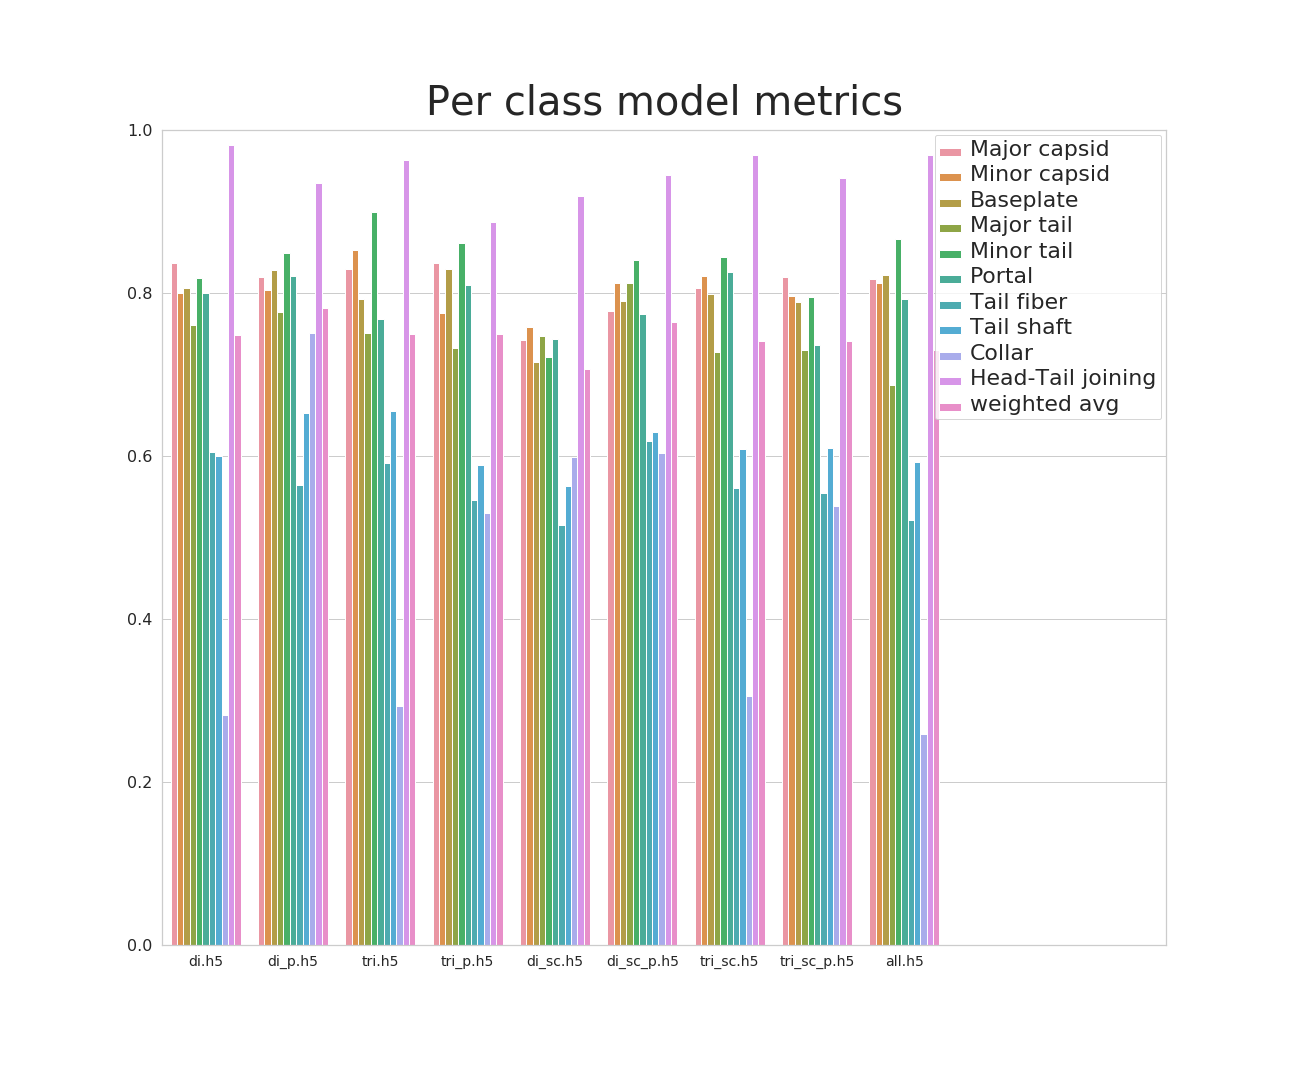
\includegraphics[width=0.90\textwidth]{f1_score}
\end{frame}

\begin{frame}{website}
\begin{center}
\qrcode{https://edwards.sdsu.edu/adrian_net}
\url{https://edwards.sdsu.edu/adrian_net}
\end{center}
\end{frame}

\begin{frame}{Conclusions}
\begin{itemize}
\item [-] ANN is slow to train but fast to run.
\item [-] Robots will rule the world
\item [-] "Collar" proteins are not a real thing
\end{itemize}
\end{frame}

\end{document}
